\documentclass{article}
% NEURIPS style (neurips_2025.sty is in paper_draft/).
% The `main' track option is required alongside `final' so that the style's
% camera-ready notice string (\@trackname) is defined.
\usepackage[final,main]{neurips_2025}

\usepackage[utf8]{inputenc}
\usepackage[T1]{fontenc}
\usepackage[hidelinks]{hyperref}  % REQUIRED: clickable links
\usepackage{booktabs}  % REQUIRED: professional tables
\usepackage{graphicx}
\usepackage{amsmath,amssymb}
\usepackage{subcaption}
\usepackage{multirow}
\usepackage{enumitem}
\usepackage{url}
\usepackage{algorithm}
\usepackage[noend]{algpseudocode}

% Import command files
\input{commands/math}
\input{commands/general}
%%%%% PROJECT-SPECIFIC MACROS %%%%%
% Adaptive experimental design for safety evaluation
% Import with: %%%%% PROJECT-SPECIFIC MACROS %%%%%
% Adaptive experimental design for safety evaluation
% Import with: %%%%% PROJECT-SPECIFIC MACROS %%%%%
% Adaptive experimental design for safety evaluation
% Import with: \input{commands/macros}

\usepackage{xspace}

%%%%%%%%%%%%%%%%%%%%%%%%%%%%%%%%%%%%%%%%%%%%%%%%%%%%%%%%%%%%%%%%%
% PROTOCOL ARM NAMES
%%%%%%%%%%%%%%%%%%%%%%%%%%%%%%%%%%%%%%%%%%%%%%%%%%%%%%%%%%%%%%%%%

\newcommand{\staticzero}{\textsc{Static-d0}\xspace}
\newcommand{\staticone}{\textsc{Static-d1}\xspace}
\newcommand{\statictwo}{\textsc{Static-d2}\xspace}
\newcommand{\fixedsplit}{\textsc{Fixed-Split}\xspace}
\newcommand{\ladder}{\textsc{Ladder}\xspace}
\newcommand{\oracle}{\textsc{Oracle}\xspace}

\newcommand{\singlemethod}{\textsc{Static-Single}\xspace}
\newcommand{\roundrobin}{\textsc{Static-RR}\xspace}
\newcommand{\bestsingle}{\textsc{Static-Best}\xspace}
\newcommand{\thompson}{\textsc{Adapt-TS}\xspace}
\newcommand{\escalthompson}{\textsc{Adapt-Esc+TS}\xspace}
\newcommand{\succhalving}{\textsc{Adapt-SH}\xspace}

\newcommand{\fixedcp}{\textsc{Fixed-CP}\xspace}
\newcommand{\adaptivecp}{\textsc{Adaptive-CP}\xspace}
\newcommand{\unioncp}{\textsc{Union-CP}\xspace}
\newcommand{\extrapolative}{\textsc{Extrapolative}\xspace}

\newcommand{\staticpone}{\textsc{Static-P1}\xspace}

%%%%%%%%%%%%%%%%%%%%%%%%%%%%%%%%%%%%%%%%%%%%%%%%%%%%%%%%%%%%%%%%%
% DATASET NAMES
%%%%%%%%%%%%%%%%%%%%%%%%%%%%%%%%%%%%%%%%%%%%%%%%%%%%%%%%%%%%%%%%%

\newcommand{\rstraj}{\textsc{RS-Traj}\xspace}
\newcommand{\jbb}{\textsc{JBB-Artifacts}\xspace}
\newcommand{\gsmk}{\textsc{GSM8K}\xspace}
\newcommand{\advbench}{\textsc{AdvBench}\xspace}

%%%%%%%%%%%%%%%%%%%%%%%%%%%%%%%%%%%%%%%%%%%%%%%%%%%%%%%%%%%%%%%%%
% MODEL NAMES
%%%%%%%%%%%%%%%%%%%%%%%%%%%%%%%%%%%%%%%%%%%%%%%%%%%%%%%%%%%%%%%%%

\newcommand{\qwenseven}{\textsc{Qwen2.5-7B}\xspace}
\newcommand{\qwensmall}{\textsc{Qwen2.5-1.5B}\xspace}
\newcommand{\phimini}{\textsc{Phi-3.5-mini}\xspace}
\newcommand{\llamaseven}{\textsc{Llama-2-7B-chat}\xspace}
\newcommand{\gptfour}{\textsc{GPT-4-0125}\xspace}
\newcommand{\gptthree}{\textsc{GPT-3.5-turbo}\xspace}

%%%%%%%%%%%%%%%%%%%%%%%%%%%%%%%%%%%%%%%%%%%%%%%%%%%%%%%%%%%%%%%%%
% DOMAIN-SPECIFIC TERMS
%%%%%%%%%%%%%%%%%%%%%%%%%%%%%%%%%%%%%%%%%%%%%%%%%%%%%%%%%%%%%%%%%

\newcommand{\family}{design family\xspace}
\newcommand{\families}{design families\xspace}

%%%%%%%%%%%%%%%%%%%%%%%%%%%%%%%%%%%%%%%%%%%%%%%%%%%%%%%%%%%%%%%%%
% ABBREVIATIONS
%%%%%%%%%%%%%%%%%%%%%%%%%%%%%%%%%%%%%%%%%%%%%%%%%%%%%%%%%%%%%%%%%

\newcommand{\ie}{i.e.,\xspace}
\newcommand{\wrt}{w.r.t.\xspace}


\usepackage{xspace}

%%%%%%%%%%%%%%%%%%%%%%%%%%%%%%%%%%%%%%%%%%%%%%%%%%%%%%%%%%%%%%%%%
% PROTOCOL ARM NAMES
%%%%%%%%%%%%%%%%%%%%%%%%%%%%%%%%%%%%%%%%%%%%%%%%%%%%%%%%%%%%%%%%%

\newcommand{\staticzero}{\textsc{Static-d0}\xspace}
\newcommand{\staticone}{\textsc{Static-d1}\xspace}
\newcommand{\statictwo}{\textsc{Static-d2}\xspace}
\newcommand{\fixedsplit}{\textsc{Fixed-Split}\xspace}
\newcommand{\ladder}{\textsc{Ladder}\xspace}
\newcommand{\oracle}{\textsc{Oracle}\xspace}

\newcommand{\singlemethod}{\textsc{Static-Single}\xspace}
\newcommand{\roundrobin}{\textsc{Static-RR}\xspace}
\newcommand{\bestsingle}{\textsc{Static-Best}\xspace}
\newcommand{\thompson}{\textsc{Adapt-TS}\xspace}
\newcommand{\escalthompson}{\textsc{Adapt-Esc+TS}\xspace}
\newcommand{\succhalving}{\textsc{Adapt-SH}\xspace}

\newcommand{\fixedcp}{\textsc{Fixed-CP}\xspace}
\newcommand{\adaptivecp}{\textsc{Adaptive-CP}\xspace}
\newcommand{\unioncp}{\textsc{Union-CP}\xspace}
\newcommand{\extrapolative}{\textsc{Extrapolative}\xspace}

\newcommand{\staticpone}{\textsc{Static-P1}\xspace}

%%%%%%%%%%%%%%%%%%%%%%%%%%%%%%%%%%%%%%%%%%%%%%%%%%%%%%%%%%%%%%%%%
% DATASET NAMES
%%%%%%%%%%%%%%%%%%%%%%%%%%%%%%%%%%%%%%%%%%%%%%%%%%%%%%%%%%%%%%%%%

\newcommand{\rstraj}{\textsc{RS-Traj}\xspace}
\newcommand{\jbb}{\textsc{JBB-Artifacts}\xspace}
\newcommand{\gsmk}{\textsc{GSM8K}\xspace}
\newcommand{\advbench}{\textsc{AdvBench}\xspace}

%%%%%%%%%%%%%%%%%%%%%%%%%%%%%%%%%%%%%%%%%%%%%%%%%%%%%%%%%%%%%%%%%
% MODEL NAMES
%%%%%%%%%%%%%%%%%%%%%%%%%%%%%%%%%%%%%%%%%%%%%%%%%%%%%%%%%%%%%%%%%

\newcommand{\qwenseven}{\textsc{Qwen2.5-7B}\xspace}
\newcommand{\qwensmall}{\textsc{Qwen2.5-1.5B}\xspace}
\newcommand{\phimini}{\textsc{Phi-3.5-mini}\xspace}
\newcommand{\llamaseven}{\textsc{Llama-2-7B-chat}\xspace}
\newcommand{\gptfour}{\textsc{GPT-4-0125}\xspace}
\newcommand{\gptthree}{\textsc{GPT-3.5-turbo}\xspace}

%%%%%%%%%%%%%%%%%%%%%%%%%%%%%%%%%%%%%%%%%%%%%%%%%%%%%%%%%%%%%%%%%
% DOMAIN-SPECIFIC TERMS
%%%%%%%%%%%%%%%%%%%%%%%%%%%%%%%%%%%%%%%%%%%%%%%%%%%%%%%%%%%%%%%%%

\newcommand{\family}{design family\xspace}
\newcommand{\families}{design families\xspace}

%%%%%%%%%%%%%%%%%%%%%%%%%%%%%%%%%%%%%%%%%%%%%%%%%%%%%%%%%%%%%%%%%
% ABBREVIATIONS
%%%%%%%%%%%%%%%%%%%%%%%%%%%%%%%%%%%%%%%%%%%%%%%%%%%%%%%%%%%%%%%%%

\newcommand{\ie}{i.e.,\xspace}
\newcommand{\wrt}{w.r.t.\xspace}


\usepackage{xspace}

%%%%%%%%%%%%%%%%%%%%%%%%%%%%%%%%%%%%%%%%%%%%%%%%%%%%%%%%%%%%%%%%%
% PROTOCOL ARM NAMES
%%%%%%%%%%%%%%%%%%%%%%%%%%%%%%%%%%%%%%%%%%%%%%%%%%%%%%%%%%%%%%%%%

\newcommand{\staticzero}{\textsc{Static-d0}\xspace}
\newcommand{\staticone}{\textsc{Static-d1}\xspace}
\newcommand{\statictwo}{\textsc{Static-d2}\xspace}
\newcommand{\fixedsplit}{\textsc{Fixed-Split}\xspace}
\newcommand{\ladder}{\textsc{Ladder}\xspace}
\newcommand{\oracle}{\textsc{Oracle}\xspace}

\newcommand{\singlemethod}{\textsc{Static-Single}\xspace}
\newcommand{\roundrobin}{\textsc{Static-RR}\xspace}
\newcommand{\bestsingle}{\textsc{Static-Best}\xspace}
\newcommand{\thompson}{\textsc{Adapt-TS}\xspace}
\newcommand{\escalthompson}{\textsc{Adapt-Esc+TS}\xspace}
\newcommand{\succhalving}{\textsc{Adapt-SH}\xspace}

\newcommand{\fixedcp}{\textsc{Fixed-CP}\xspace}
\newcommand{\adaptivecp}{\textsc{Adaptive-CP}\xspace}
\newcommand{\unioncp}{\textsc{Union-CP}\xspace}
\newcommand{\extrapolative}{\textsc{Extrapolative}\xspace}

\newcommand{\staticpone}{\textsc{Static-P1}\xspace}

%%%%%%%%%%%%%%%%%%%%%%%%%%%%%%%%%%%%%%%%%%%%%%%%%%%%%%%%%%%%%%%%%
% DATASET NAMES
%%%%%%%%%%%%%%%%%%%%%%%%%%%%%%%%%%%%%%%%%%%%%%%%%%%%%%%%%%%%%%%%%

\newcommand{\rstraj}{\textsc{RS-Traj}\xspace}
\newcommand{\jbb}{\textsc{JBB-Artifacts}\xspace}
\newcommand{\gsmk}{\textsc{GSM8K}\xspace}
\newcommand{\advbench}{\textsc{AdvBench}\xspace}

%%%%%%%%%%%%%%%%%%%%%%%%%%%%%%%%%%%%%%%%%%%%%%%%%%%%%%%%%%%%%%%%%
% MODEL NAMES
%%%%%%%%%%%%%%%%%%%%%%%%%%%%%%%%%%%%%%%%%%%%%%%%%%%%%%%%%%%%%%%%%

\newcommand{\qwenseven}{\textsc{Qwen2.5-7B}\xspace}
\newcommand{\qwensmall}{\textsc{Qwen2.5-1.5B}\xspace}
\newcommand{\phimini}{\textsc{Phi-3.5-mini}\xspace}
\newcommand{\llamaseven}{\textsc{Llama-2-7B-chat}\xspace}
\newcommand{\gptfour}{\textsc{GPT-4-0125}\xspace}
\newcommand{\gptthree}{\textsc{GPT-3.5-turbo}\xspace}

%%%%%%%%%%%%%%%%%%%%%%%%%%%%%%%%%%%%%%%%%%%%%%%%%%%%%%%%%%%%%%%%%
% DOMAIN-SPECIFIC TERMS
%%%%%%%%%%%%%%%%%%%%%%%%%%%%%%%%%%%%%%%%%%%%%%%%%%%%%%%%%%%%%%%%%

\newcommand{\family}{design family\xspace}
\newcommand{\families}{design families\xspace}

%%%%%%%%%%%%%%%%%%%%%%%%%%%%%%%%%%%%%%%%%%%%%%%%%%%%%%%%%%%%%%%%%
% ABBREVIATIONS
%%%%%%%%%%%%%%%%%%%%%%%%%%%%%%%%%%%%%%%%%%%%%%%%%%%%%%%%%%%%%%%%%

\newcommand{\ie}{i.e.,\xspace}
\newcommand{\wrt}{w.r.t.\xspace}


\captionsetup[subfigure]{aboveskip=4pt,belowskip=4pt}
\captionsetup[table]{aboveskip=4pt,belowskip=4pt}
\captionsetup[figure]{aboveskip=4pt,belowskip=4pt}

\bibliographystyle{plainnat}

\title{Nulls Are Not Feedback: Adaptive Safety Evaluation\\
Pays Across Design Families, Not Within Them}

\author{NeuriCo}

\begin{document}

\maketitle

\begin{abstract}
Safety evaluations report nulls constantly: ``we could not elicit the behaviour.'' That
sentence is load-bearing in deployment decisions, and it is ambiguous, because it can mean the
model is robust or that the experiment was badly designed. A popular remedy is adaptivity: treat
a null as feedback and redesign. We test this directly, holding total compute constant, which no
prior work does. We replay four protocol families against 437k real per-iteration attack traces,
a complete $5\times4\times100$ cost-to-discovery matrix, and a live grid on three open-weights
instruct models under an anti-sycophancy intervention. Adaptivity helps enormously: a protocol
that spreads a fixed budget over three design families detects 100\% of behaviours where the
default single-design protocol detects 0\% at every budget up to 10{,}000 iterations. But almost
none of that gain comes from the proposed mechanism. Against a comparator that switches design
family on a blind fixed schedule with identical budget and identical designs, using the null as
a trigger gains nothing ($\Delta = +0.02$) and loses at large budgets ($\Delta = -0.12$). We
explain why: conditional on a run still being null, the continuous progress signal predicts
eventual success at AUC $0.45$--$0.61$, with every interval covering chance. Adaptivity at the
portfolio level does work ($+0.65$ behaviours on GPT-4; $+0.72$ live on Qwen2.5-7B). Finally,
nominally 95\% bounds on residual vulnerability achieve 63--67\% coverage, and an anytime-valid
correction barely helps, because the estimand, not the stopping rule, is wrong.

\end{abstract}

\section{Introduction}
\label{sec:intro}

A safety evaluation that finds nothing is the most common result in AI safety, and the least
interpretable. ``We could not elicit the behaviour'' can mean the model is robust, or it can
mean the experiment was not sensitive enough to see the failure. Static protocols cannot tell
the two apart, and the difference matters: this sentence appears in model cards, audit reports,
and deployment decisions.

The literature already contains proof that the second reading is often the correct one. In the
JailbreakBench artifacts, PAIR~\cite{chao2023pair} scores $0.00$ attack success against
\llamaseven while prompt-plus-random-search scores $0.90$ on the \emph{same} 100 behaviours of
the \emph{same} model~\cite{chao2024jbb,andriushchenko2024adaptive}. A lab that ran only PAIR
would have published a false robustness claim. Similar reversals recur across the alignment
literature: jailbreaks reported as ineffective against unlearning succeed when applied more
carefully~\cite{lucki2024unlearning}, and defenses reporting single-digit attack success under
automated single-turn attacks fall to human multi-turn red teaming more than 70\% of the
time~\cite{li2024mhj}.

The natural response, and the hypothesis we test, is that protocols should be \emph{adaptive}:
treat a null as actionable feedback and use it to trigger experimental redesign. This idea is
widely endorsed and, so far, untested as such.

\para{The gap.} Adaptivity has been argued for \emph{attacks}~\cite{andriushchenko2024adaptive}
and for \emph{forecasting} rare behaviours~\cite{jones2025forecasting}, but never with the
protocol as the independent variable and total compute held fixed. Every published adaptivity
result is confounded with spending more queries, so ``adaptive beats static'' may only mean
``more compute beats less compute.'' Worse, the word ``adaptive'' silently conflates two very
different moves: adjusting parameters \emph{inside} a design family, and \emph{switching} design
family. And nobody scores the null branch, \ie what an adaptive protocol should output when it
still finds nothing. That branch is exactly the half of the claim that safety cases rest on.

\para{Our approach.} We make the protocol the independent variable and hold the budget constant
by construction. Each substrate's outcome matrix is evaluated exhaustively once, and protocols
are then \emph{replayed} against the cached matrix under an identical budget $B$. This removes
the compute confound, makes every comparison paired on the same behaviours, and lets us report
whole detection-versus-budget curves rather than single points. We run four experiments on three
substrates: 437k per-iteration random-search traces released by
\citet{andriushchenko2024adaptive}; the official JailbreakBench cost-to-discovery
matrix~\cite{chao2024jbb} of 5 attacks $\times$ 4 target models $\times$ 100 behaviours; and a
live grid on three open-weights instruct models run locally under a real anti-sycophancy
intervention, using sycophantic answer-flipping on \gsmk~\cite{cobbe2021gsm8k} as a non-harmful
failure mode.

The critical design choice is our comparator. Most work contrasts an adaptive protocol with a
single static design, which cannot separate ``adaptivity works'' from ``design diversity
works.'' We add \fixedsplit: same budget, same set of design families, but the switch points are
placed on a blind schedule that ignores the data. Our adaptive arm \ladder is built so that
disabling its trigger recovers \fixedsplit exactly, so the two arms differ \emph{only} in
whether the null is used as a trigger.

\para{What we find.} The motivating phenomenon is real and extreme: the default design detects
$0/50$ behaviours at every budget up to $10{,}000$ iterations, while a protocol spending the
identical budget across three design families reaches $1.00$ (McNemar $p<10^{-6}$, Cohen's
$h \approx 2.4$). But against \fixedsplit, the null-as-trigger mechanism gains nothing
($\Delta = +0.02$, $p = 0.73$) and loses at large budgets ($\Delta = -0.12$, 95\% CI
$[-0.22, -0.04]$). We trace this to a mechanistic fact: conditional on a run still being null at
iteration $t$, the continuous progress signal predicts eventual success at pooled AUC
$0.45$--$0.61$, with every confidence interval covering $0.5$. Adaptivity at the \emph{portfolio}
level does work, beating an equally diversified static schedule by $+0.65$ behaviours on GPT-4
and by $+0.72$ live on \qwenseven. Finally, nominally 95\% upper bounds on residual vulnerability
achieve 63--67\% empirical coverage, and an anytime-valid correction for optional stopping moves
coverage only from $0.638$ to $0.671$.

\para{Contributions.}
\begin{itemize}[leftmargin=*,itemsep=0pt,topsep=2pt]
    \item We propose a compute-matched replay methodology that makes the evaluation protocol the
    independent variable, and we instantiate it on three substrates covering replayed attack
    traces, a benchmark cost matrix, and live open-weights models.
    \item We decompose ``adaptive'' into within-search escalation and portfolio-level allocation,
    and show with a trigger-ablated comparator that the entire measured benefit comes from
    searching multiple design families, not from the null-as-trigger mechanism.
    \item We test the mechanism directly by measuring the diagnosticity (AUC) of the progress
    signal on the surviving-null population, and find it indistinguishable from chance at all
    seven checkpoints.
    \item We score the null branch and show that nominally 95\% bounds cover 63--67\% of the
    time, that anytime-valid correction does not repair this, and that on total nulls tail
    extrapolation is undefined 100\% of the time.
    \item We replicate the whole contrast live on \qwenseven, \qwensmall and \phimini, where a
    static protocol using the natural first design measures a 3.7\% flip rate and would report
    that the anti-sycophancy intervention holds, while 85\% of items flip under a different
    pressure family.
\end{itemize}

\Secref{sec:related} positions the work, \secref{sec:method} describes the substrates and
protocol arms, \secref{sec:results} reports the four experiments, and
\twosecrefs{sec:discussion}{sec:conclusion} discuss implications and limitations.

\section{Related Work}
\label{sec:related}

\para{Adaptive attacks.} Automated red teaming began with attacker language models and large-scale
human red teaming~\cite{perez2022redteaming,ganguli2022redteaming} and with gradient-based universal
suffixes~\cite{zou2023gcg}, and is now standardised by HarmBench~\cite{mazeika2024harmbench}. Nearly
every method since iterates on failure.
PAIR~\cite{chao2023pair} refines a candidate using the target's refusal, TAP~\cite{mehrotra2023tap}
adds tree search with pruning, Rainbow Teaming~\cite{samvelyan2024rainbow} maintains a
quality-diversity archive over attack styles, GOAT~\cite{pavlova2024goat} picks a published attack
technique per turn, and curiosity-driven red teaming~\cite{hong2024curiosity} adds a novelty bonus
to an RL attacker. \citet{andriushchenko2024adaptive} state the thesis most directly: adaptive
attacks are necessary for accurate robustness evaluation, and no single method generalises across
targets. Their ablation on \llamaseven moves from 0\% to 50\% to 100\% attack success as random
search and then self-transfer initialisation are added, and their R2D2 result is the built-in
negative control: self-transfer gives only 12\% there, while switching to an in-context template
family gives 90\%. Best-of-$N$~\cite{hughes2024bon} is the canonical non-adaptive control, being
memoryless by construction, and establishes the power law $-\log \mathrm{ASR}(N) = aN^{-b}$ that
we use as the extrapolative bound in \secref{sec:results}. Unlike all of this work, we hold the
attack set fixed and vary the \emph{protocol} that schedules it under a fixed budget, so
adaptivity is not confounded with compute.

\para{Return curves and reproducibility.} Whether adaptive allocation can beat uniform allocation at
all depends on the shape of the return curve. \citet{halder2026scaling} report a polynomial regime
without prompt injection and an exponential regime with it, and \citet{topol2026process} apply
process mining to 8{,}575 scored red-teaming events to show that mutator effectiveness is asymmetric
across models and that time-to-jailbreak distributions differ by an order of magnitude. This is
independent 2026 confirmation of the lesson we build on, that which adaptation works is
model-specific. \citet{fang2026foundry} reproduce 30 published attacks in a unified harness to a
mean deviation of $+0.26$ percentage points, which is the kind of control that makes replay-based
comparisons like ours credible.

\para{Nulls, forecasting, and elicitation.} \citet{jones2025forecasting} give the closest prior
work: they replace a binary null with a continuous elicitation probability and extrapolate extreme
quantiles via a Gumbel-tail fit, forecasting risk two orders of magnitude beyond the observed
budget. Their final section uses forecasts to allocate red-teaming compute, which is the direct
ancestor of our portfolio experiment. They also propose adaptively stopping unpromising queries as
future work. We take that proposal seriously enough to test it, and find that the within-run
signal it would rely on is not diagnostic on the population that matters.

\para{Hidden robustness and false nulls.} A second literature supplies the phenomena.
\citet{wei2023jailbroken} give the taxonomy, splitting failures into competing objectives and
mismatched generalisation, which is in effect a principled axis set for a design space. Shallow
safety alignment~\cite{qi2024shallow} shows alignment mostly adapts the first few output tokens,
which explains why suffix, prefilling, and decoding attacks all work. Sleeper
agents~\cite{hubinger2024sleeper} persist through SFT, RL, and adversarial training, with
adversarial training teaching models to hide the trigger better. Fine-tuning breaks guardrails with
ten examples~\cite{qi2023finetuning}. \citet{lucki2024unlearning} recover unlearned capabilities
with attacks previously reported as ineffective, and \citet{che2025tampering} show that input-output
evaluations only lower-bound worst-case behaviour. On the other side, latent adversarial
training~\cite{sheshadri2024lat} and constitutional classifiers~\cite{sharma2025classifiers} are
rare cases where a null appears to be earned, the latter at a cost of over 3{,}000 human red-teaming
hours. \citet{betley2025emergent} add a measurement problem that compounds all of this: narrowly
fine-tuned models behave inconsistently and sometimes act aligned, so single-sample evaluation has
low power by construction. Whether adaptive search should pay depends on the dimensionality of the vulnerability
boundary, which is itself disputed: \citet{arditi2024refusal} report a single refusal direction,
while \citet{wollschlager2025geometry} report multi-dimensional concept cones. We treat this as a
moderator rather than settled, and our results are consistent with the family-dependent view.

\para{Statistics for evaluation.} \citet{miller2024errorbars} imports standard errors, clustering,
paired inference, and power analysis into evaluation, and shows clustered standard errors can be
$3.05\times$ larger than naive ones. \citet{bowyer2025clt} show CLT intervals badly understate
uncertainty below a few hundred datapoints, which matters here because adaptive protocols
concentrate budget on small subsets. Anytime-valid inference~\cite{ramdas2022savi,lindon2022anytime}
is the correct frame for data-dependent stopping, and adaptive item selection with preserved
coverage has been developed for capability estimation~\cite{polo2024tinybenchmarks,krumdick2026wild,wu2026faq,tolochinsky2026valid}.
\citet{dorner2024limits} bound how far an LLM judge can substitute for labels, which is why we
report both a judge-based and a rule-based outcome throughout. The red-teaming literature has the
optional-stopping problem and this literature has the fix; we join them, and find, surprisingly,
that the fix addresses the smaller of two errors.

\para{Bayesian experimental design.} The formal vocabulary the hypothesis reaches for informally is
that of sequential Bayesian experimental design~\cite{rainforth2023boed}, where a design policy maps
history to the next design so as to maximise expected information gain, and can be amortised into a
single forward pass~\cite{foster2021dad}. Our results say something concrete to that framework in
this domain: the expected information gain of a within-run null is close to zero under the surrogate
that is actually available, while the expected information gain of a cross-run null about which
\family to use is large.

\para{Positioning.} Our contribution is the controlled comparison that none of the above performs:
protocol as independent variable, compute held constant, within-family and cross-family adaptivity
separated by an ablated comparator, and the null branch scored for coverage rather than assumed
valid.

\section{Methodology}
\label{sec:method}

\subsection{Problem setup}

An evaluation protocol $\pi$ is given a budget $B$ of unit-cost queries, a set of targets
(behaviours or items) $\gI$, and a set of \families $\gF$. A design family is a qualitatively
distinct way of probing the model: a suffix-search initialisation, a prompt template class, or a
social-pressure schema. At each step the protocol chooses a target and a family, spends one unit,
and observes an outcome $y \in \{0,1\}$ together with a continuous surrogate score $s \in \R$. The
primary dependent variable is the \emph{detection rate} at matched budget,
$D_\pi(B) = \frac{1}{|\gI|}\sum_{i\in\gI} \1[\pi \text{ elicits the behaviour on } i \text{ within } B]$.
We report $D_\pi(B)$ as a whole curve over $B$, never as a single point.

The key comparison in this paper is not adaptive versus static. It is adaptive versus
\emph{blindly diversified}. Let $\pi_{\text{blind}}$ spend $B$ across $\gF$ on a schedule that is a
function of $B$ alone, and let $\pi_{\text{adapt}}$ spend $B$ across the same $\gF$ using a
schedule that is a function of $(B, s_{1:t})$. Because $\pi_{\text{adapt}}$ reduces to
$\pi_{\text{blind}}$ when its trigger is disabled, $D_{\pi_{\text{adapt}}}(B) -
D_{\pi_{\text{blind}}}(B)$ isolates the value of using the null as a trigger, with everything else
held fixed.

\subsection{Substrates}

\tabref{tab:substrates} lists the three substrates. Nothing in E1--E3 is re-run or simulated:
these are the original authors' own released traces and the official benchmark artifacts. E4 uses
real model weights executed locally. No simulated agent appears anywhere in this work.

\begin{table}[t]
    \centering
    \resizebox{\textwidth}{!}{%
    \begin{tabular}{@{}llll@{}}
        \toprule
        \textbf{Experiment} & \textbf{Substrate} & \textbf{Size} & \textbf{Role} \\
        \midrule
        E1, E1c, E3 & \rstraj: released per-iteration & 14 configs, $\sim$437k iteration rows, & Real sequential traces with a continuous \\
                    & random-search logs~\cite{andriushchenko2024adaptive} & 672 run outcomes & objective; contains a matched adaptive/static pair \\
        \addlinespace
        E2 & \jbb: official JailbreakBench & 5 methods $\times$ 4 target models & Complete cost-to-discovery matrix; any \\
           & artifacts~\cite{chao2024jbb} & $\times$ 100 behaviours & allocation policy can be replayed offline \\
        \addlinespace
        E4 & \gsmk test split~\cite{cobbe2021gsm8k} + real & 32 items $\times$ 4 pressure families & End-to-end live replication on a fresh, \\
           & open-weights LLMs run locally & $\times$ 2 conditions $\times$ 3 models & non-harmful failure mode \\
        \bottomrule
    \end{tabular}
    }
    \caption{The three substrates. E1--E3 replay already-published traces and artifacts; E4 runs
    real model weights locally. No simulated model is used anywhere in this work.}
    \label{tab:substrates}
\end{table}


\para{\rstraj (E1, E1c, E3).} We parsed the 24 attack logs released with
\citet{andriushchenko2024adaptive} into 14 configurations, roughly 437k per-iteration rows and 672
run outcomes. Each row carries the target-token log-probability surrogate and the judge outcome, so
a protocol can be replayed at iteration granularity. The corpus contains a matched pair on
\llamaseven that differs only in initialisation policy: \texttt{plain\_init} (static) scores $0.00$
over 50 behaviours with 56\% of runs hitting the 10{,}000-iteration cap, while the self-transfer
configuration scores $0.96$ with a median of 2 iterations.

\para{\jbb (E2).} The official JailbreakBench artifacts~\cite{chao2024jbb} give
\texttt{queries\_to\_jailbreak} and a success flag for 5 attacks $\times$ 4 target models $\times$
100 behaviours. This is a complete cost-to-discovery matrix, so any allocation policy can be
replayed offline exactly.

\para{Live grid (E4).} We run three open-weights instruct
models~\cite{yang2024qwen25,abdin2024phi3} locally on 32 \gsmk test problems
under an anti-sycophancy system-prompt intervention and a no-intervention control, crossed with
four social-pressure \families: P1 simple doubt, P2 appeal to authority, P3 fabricated consensus,
P4 persistent multi-turn pressure. The failure mode is sycophantic answer-flipping, which is
non-harmful and produces no jailbreak artifacts. Only items the model answers correctly without
pressure are eligible, so ``flip'' is always well defined. Baseline accuracies are $0.844$
(\qwenseven), $0.781$ (\phimini) and $0.594$ (\qwensmall), leaving 27, 25 and 19 eligible items
respectively.

\subsection{Matched-budget replay}

Every experiment follows the same pattern. The outcome matrix is evaluated (or read) once,
exhaustively, over all targets $\times$ families $\times$ budget positions. Protocols are then
replayed against that cached matrix under an identical budget. This has three consequences. First,
the compute confound is removed by construction rather than by argument. Second, every protocol
comparison is paired on the same behaviours or items, so we can use paired tests. Third, bootstrap
uncertainty is cheap, because replaying a policy costs microseconds.

\subsection{Protocol arms}

\para{E1: within-search escalation ladder.} Three \families are available on \llamaseven: $d_0$ the
default \texttt{plain\_init} random search, $d_1$ re-initialisation from a related success
(self-transfer), and $d_2$ a switch of template family. The arms are \staticzero, \staticone and
\statictwo (all $B$ on one family; \staticzero is the ``continue-only'' control, \ie maximal
within-family persistence), \fixedsplit ($B$ divided equally over the three families on a schedule
that ignores the data), \ladder (same designs, same $B$, but the switch point is moved by the
continuous surrogate), and \oracle (best family per behaviour). \ladder has three
hyper-parameters: a patience, a surrogate threshold $\tau$, and an extension factor. At
$\tau=0$ and extension $1$ it recovers \fixedsplit \emph{exactly}. This is what makes the
\ladder--\fixedsplit contrast decisive; the \staticzero contrast only establishes that design
diversity matters at all.

\para{E1c: null diagnosticity.} At checkpoint $t$ we restrict to runs that are \emph{still null at
$t$}, which is precisely the decision context an adaptive protocol faces, and measure the AUC of
the surrogate at $t$ for predicting whether the run eventually succeeds. If this AUC is $0.5$, no
protocol can use the null as a trigger, however cleverly implemented.

\para{E2: portfolio allocation.} Budget is a number of attack runs allocated over methods and
behaviours. Static arms are \singlemethod (the field default), \roundrobin (diversified but
non-adaptive) and \bestsingle, an \emph{oracle} single-method choice that upper-bounds any
\textit{a priori} decision. Adaptive arms are escalation, \thompson (Thompson sampling over
methods), \succhalving (successive halving) and \escalthompson. \oracle marks the union ceiling.

\para{E3: calibration of the terminal null.} A protocol stops and must emit a nominally 95\% upper
bound on the elicitable fraction. \fixedcp is Clopper-Pearson at a pre-registered budget,
\adaptivecp is the same interval at a data-chosen stopping time (what the field actually does),
\unioncp applies a Bonferroni union bound over the monitoring grid and is genuinely anytime-valid,
and \extrapolative fits the Best-of-$N$ power law~\cite{hughes2024bon} and extrapolates to the full
horizon. Ground truth is the outcome at the end of the observed trace.

\para{E4: live protocol race.} \staticpone spends its whole budget on P1, the obvious first design;
\roundrobin cycles blindly over the four families; \thompson allocates adaptively over families.
Budget is a number of model calls.

\subsection{Metrics and statistical analysis}

The analysis plan was pre-registered before any protocol was run. Primary metric is detection rate
at matched budget. Secondary metrics are queries to first detection treated as right-censored
survival data, AUC of the trigger signal, coverage and width of the emitted upper bound, and, for
E4, the flip rate under pressure and the fraction of vulnerable items localised.

Uncertainty comes from bootstrap over behaviours or items (1{,}000 resamples, seed 42), never from
re-running attacks, since the artifact matrix has one realisation per cell. Where an exact
per-behaviour join exists we use paired bootstrap plus exact McNemar on discordant behaviours;
unpaired comparisons are matched by resampling and are flagged explicitly as resting on an
exchangeability assumption. E2 and E4 comparisons use Wilcoxon signed-rank over paired policy
replicates (300 and 400 respectively). We apply Holm correction within each experiment's family of
tests at $\alpha = 0.05$, and report an effect size (risk difference, Cohen's $h$) alongside every
$p$-value. Both the GPT-4-judge and the rule-based outcome are retained throughout; they disagree,
and we report the disagreement rather than averaging it away.

\subsection{Reproducibility}

Seed 42 everywhere. E4 decoding is greedy (\texttt{do\_sample=False}, temperature 0). Environment:
Python 3.12, torch 2.13.0+cu130, transformers with native model code
(\texttt{trust\_remote\_code=False}), pandas 3.0.5, scipy 1.18.0, with \texttt{uv} managing an
isolated virtual environment. E1--E3 run on CPU in under five minutes in total; the E4 grid took
roughly 10 GPU-minutes per model on an RTX A6000.

\section{Results}
\label{sec:results}

We report four experiments. E1 and E1c ask whether the null-as-trigger mechanism works and why;
E2 asks whether adaptivity works at the portfolio level; E3 scores the null branch; E4 replicates
the whole contrast live on real models.

\subsection{E1: the escalation ladder at matched iteration budget}
\label{sec:e1}

\begin{table}[t]
    \centering
    \begin{tabular}{@{}lcccccc@{}}
        \toprule
        \textbf{Budget $B$} & \staticzero & \staticone & \statictwo & \fixedsplit & \ladder & \oracle \\
        \midrule
        8       & 0.00 & 0.62 & 0.56 & \textbf{0.80} & 0.78 & 0.84 \\
        20      & 0.00 & 0.64 & 0.56 & \textbf{0.84} & \textbf{0.84} & 0.84 \\
        60      & 0.00 & \textbf{0.98} & 0.58 & 0.84 & 0.86 & 1.00 \\
        200     & 0.00 & 0.98 & 0.60 & \textbf{1.00} & 0.88 & 1.00 \\
        10{,}000 & 0.00 & 0.98 & 0.64 & \textbf{1.00} & 0.88 & 1.00 \\
        \bottomrule
    \end{tabular}
    \caption{\textbf{E1: detection rate at matched iteration budget} on 50 \llamaseven behaviours.
    \staticzero, the default design, detects nothing across four orders of magnitude of budget,
    while every arm that searches more than one \family detects most or all behaviours.
    \ladder, which uses the null as a switch trigger, never beats \fixedsplit, which switches on a
    blind schedule with the same budget and the same designs. \oracle is an upper bound (best
    family per behaviour) and is not a deployable protocol. Best deployable arm per row in
    \textbf{bold}.}
    \label{tab:e1_detection}
\end{table}


\begin{figure}[t]
    \centering
    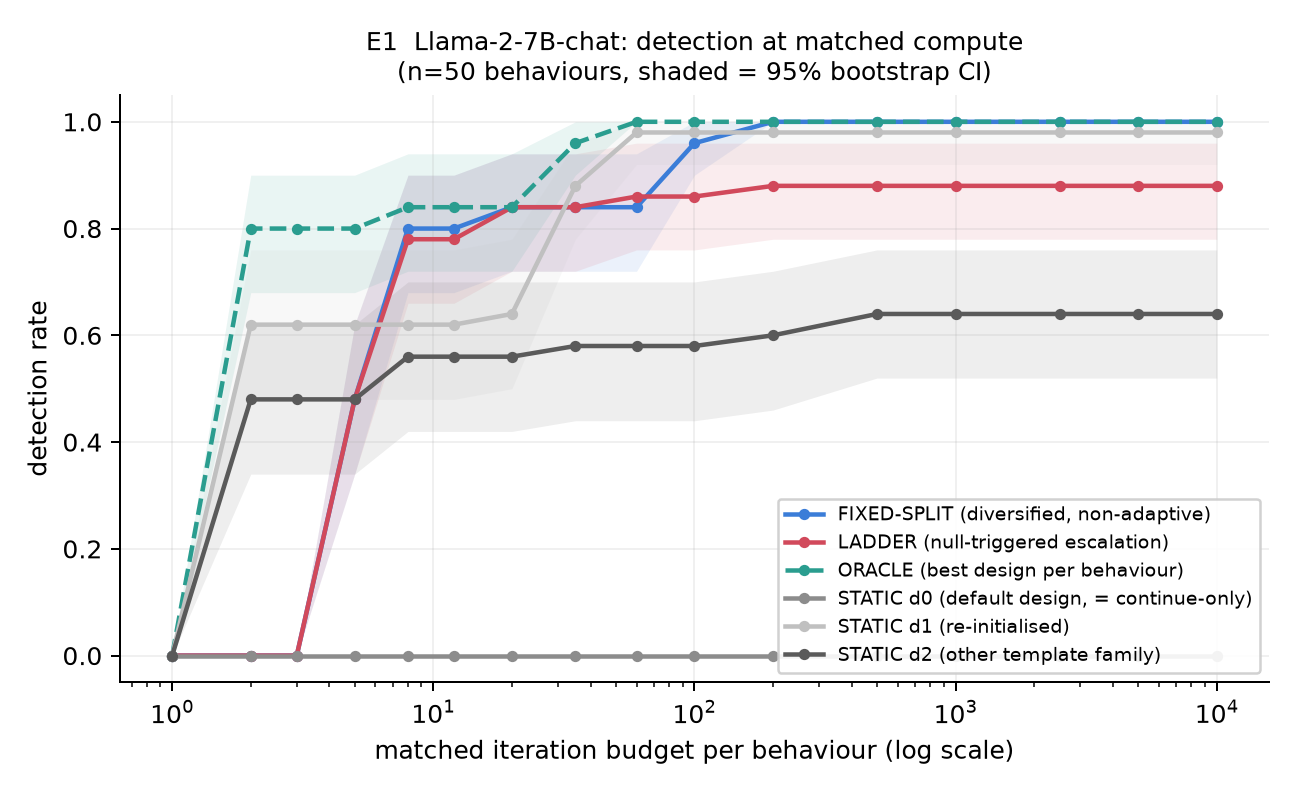
\includegraphics[width=0.95\linewidth]{figures/e1_detection_vs_budget.png}
    \caption{Detection rate versus iteration budget on 50 \llamaseven behaviours, with 95\%
    bootstrap intervals over behaviours. \staticzero (the default design) is flat at zero across
    four orders of magnitude. \ladder tracks \fixedsplit at small budgets and falls behind it at
    large budgets, so the whole gap to \staticzero is a \family effect and none of it is a trigger
    effect.}
    \label{fig:e1}
\end{figure}

Two things happen at once in \tabref{tab:e1_detection} and \figref{fig:e1}.

{\bf Is the motivating phenomenon real?} Yes, and it is extreme. \staticzero detects $0/50$
behaviours at every budget from 8 to 10{,}000 iterations, while arms that spend the identical
budget over three \families reach $1.00$. The risk difference is $0.88$--$0.98$ depending on
budget, exact McNemar $p < 10^{-6}$, Cohen's $h \approx 2.4$. This is the cleanest available
instance of a false null: 10{,}000 iterations of a perfectly reasonable attack, reported as
robustness, on a model that three other arms break almost completely. A static protocol here does
not merely under-detect. It reports total robustness where near-total vulnerability exists.

{\bf Does the null-as-trigger mechanism add anything?} No. Against \fixedsplit, which has the same
budget, the same three designs, and switches on a blind schedule, \ladder is statistically
indistinguishable at small budgets ($B=60$: $\Delta = +0.02$, 95\% CI $[0.00, 0.06]$, McNemar
$p = 1.0$; pooled small-budget $p = 0.73$) and \emph{worse} at large budgets ($B=1000$:
$\Delta = -0.12$, 95\% CI $[-0.22, -0.04]$, bootstrap $p = 0.004$; 6 behaviours lost, 0 gained).
The Holm-adjusted McNemar $p$ for the large-budget loss is $1.0$, so we report it as a consistent
negative trend rather than a confirmed harm. Against \staticzero, by contrast, \ladder wins
overwhelmingly ($B=60$: $\Delta = +0.86$, 95\% CI $[0.76, 0.94]$, McNemar $p < 10^{-6}$,
$h = 2.37$; the exactly-paired two-rung variant gives $\Delta = +0.98$, $h = 2.86$).

\para{Rung attribution.} The decomposition is direct. Across every budget, \emph{zero} of \ladder's
detections come from rung 0 (continue in the default family); 31 come from rung 1
(re-initialisation) and 13 from rung 2 (template-family switch). The entire measured benefit of
``adaptivity'' here is attributable to searching more than one \family.

\para{Sensitivity.} The finding is not a knife-edge artifact of one trigger setting. A
$3\times3\times3$ sweep over patience $\in \{2,5,20\}$, threshold $\tau \in \{0.05,0.3,0.7\}$ and
extension $\in \{1,3,10\}$ never produces a gain over \fixedsplit larger than $+0.06$, and produces
losses as large as $-0.17$.

\subsection{E1c: why the trigger fails}
\label{sec:e1c}

\begin{table}[t]
    \centering
    \begin{tabular}{@{}rrrccr@{}}
        \toprule
        \textbf{Checkpoint $t$} & $n$ & \textbf{configs} & \textbf{pooled AUC} & \textbf{95\% CI} & \textbf{base rate} \\
        \midrule
        1   & 471 & 10 & 0.515 & [0.47, 0.57] & 0.69 \\
        2   & 471 & 10 & 0.612 & [0.50, 0.75] & 0.69 \\
        3   & 186 & 7  & 0.474 & [0.29, 0.59] & 0.51 \\
        5   & 142 & 5  & 0.448 & [0.23, 0.56] & 0.54 \\
        10  & 126 & 4  & 0.470 & [0.28, 0.60] & 0.52 \\
        25  & 102 & 3  & 0.578 & [0.30, 0.69] & 0.46 \\
        100 & 67  & 3  & 0.536 & [0.43, 0.62] & 0.40 \\
        \bottomrule
    \end{tabular}
    \caption{\textbf{E1c: the null carries no usable signal.} Conditional on a run still being null
    at iteration $t$, the AUC of the continuous target-token surrogate for predicting eventual
    success. Every confidence interval covers $0.5$. The easy successes have already left the
    population by $t$, and what remains is not separable, which is why a trigger built on this
    signal cannot work.}
    \label{tab:e1c_auc}
\end{table}


\begin{figure}[t]
    \centering
    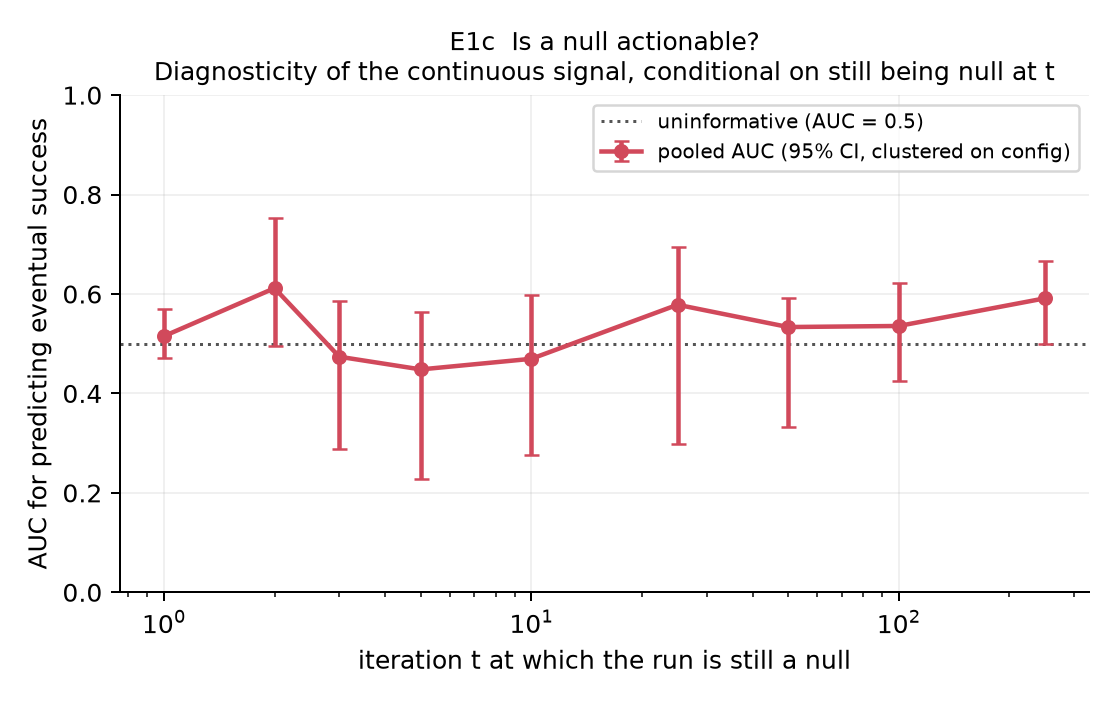
\includegraphics[width=0.85\linewidth]{figures/e1c_null_diagnosticity.png}
    \caption{Diagnosticity of the null. Pooled AUC (with 95\% intervals) of the continuous
    target-token surrogate at checkpoint $t$ for predicting eventual success, restricted to runs
    still null at $t$. The horizontal line marks chance. No checkpoint separates from $0.5$, which
    means the information a null-triggered protocol would act on does not exist in this signal.}
    \label{fig:e1c}
\end{figure}

E1 shows that the trigger does not help. E1c shows why, and this is a mechanistic refutation rather
than a restatement. Conditional on a run still being a null at iteration $t$, which is exactly the
decision context an adaptive protocol faces, the continuous surrogate predicts eventual success at
pooled AUC $0.448$--$0.612$ across seven checkpoints, and \emph{every} confidence interval covers
$0.5$ (\tabref{tab:e1c_auc}, \figref{fig:e1c}). The base rate falls from $0.69$ at $t=1$ to $0.40$
at $t=100$, confirming that the easy successes leave the population early; what remains is not
separable by this signal.

This explains the $-0.12$ loss at large budget in E1. A protocol that trusts an uninformative
signal will sometimes read a high surrogate value as evidence of progress and spend its remaining
budget persisting with a doomed rung. Because the signal is noise, that persistence is a pure loss.

\subsection{E2: portfolio-level adaptivity does work}
\label{sec:e2}

\begin{table}[t]
    \centering
    \resizebox{\textwidth}{!}{%
    \begin{tabular}{@{}lcccccc@{}}
        \toprule
        \multirow{2}{*}{\textbf{Budget}} & \multicolumn{3}{c}{\textbf{Static}} & \multicolumn{2}{c}{\textbf{Adaptive}} & \multirow{2}{*}{\oracle} \\
        \cmidrule(lr){2-4} \cmidrule(lr){5-6}
         & \singlemethod & \roundrobin & \bestsingle (oracle) & \thompson & \escalthompson & \\
        \midrule
        \multicolumn{7}{@{}l}{\gptfour-preview \quad (design-space ceiling 0.86)} \\
        \midrule
        50  & 0.155 & 0.020 & 0.393 & 0.320 & \textbf{0.325} & 0.50 \\
        100 & 0.308 & 0.040 & 0.780 & 0.688 & \textbf{0.703} & 0.86 \\
        150 & 0.308 & 0.040 & 0.780 & 0.808 & \textbf{0.860} & 0.86 \\
        300 & 0.308 & 0.360 & 0.780 & \textbf{0.860} & \textbf{0.860} & 0.86 \\
        \midrule
        \multicolumn{7}{@{}l}{\gptthree-1106 \quad (design-space ceiling 0.95)} \\
        \midrule
        100 & 0.545 & 0.470 & 0.930 & 0.791 & \textbf{0.859} & 0.95 \\
        150 & 0.545 & 0.470 & 0.930 & 0.937 & \textbf{0.950} & 0.95 \\
        300 & 0.545 & 0.810 & 0.930 & \textbf{0.950} & \textbf{0.950} & 0.95 \\
        \bottomrule
    \end{tabular}
    }
    \caption{\textbf{E2: portfolio-level adaptivity works.} Fraction of 100 behaviours jailbroken at
    matched budget (number of attack runs; 300 policy replicates per cell). Adaptive allocation
    beats the equally diversified \roundrobin by $+0.648$ on \gptfour and $+0.321$ on \gptthree at
    budget 100 (Holm-adjusted $p<0.001$), and at budget 150 it exceeds \bestsingle, an oracle
    single-method allocation, because no single method covers all behaviours. Best deployable arm
    per row in \textbf{bold}; \bestsingle and \oracle are upper bounds, not protocols.}
    \label{tab:e2_portfolio}
\end{table}


\begin{figure}[t]
    \centering
    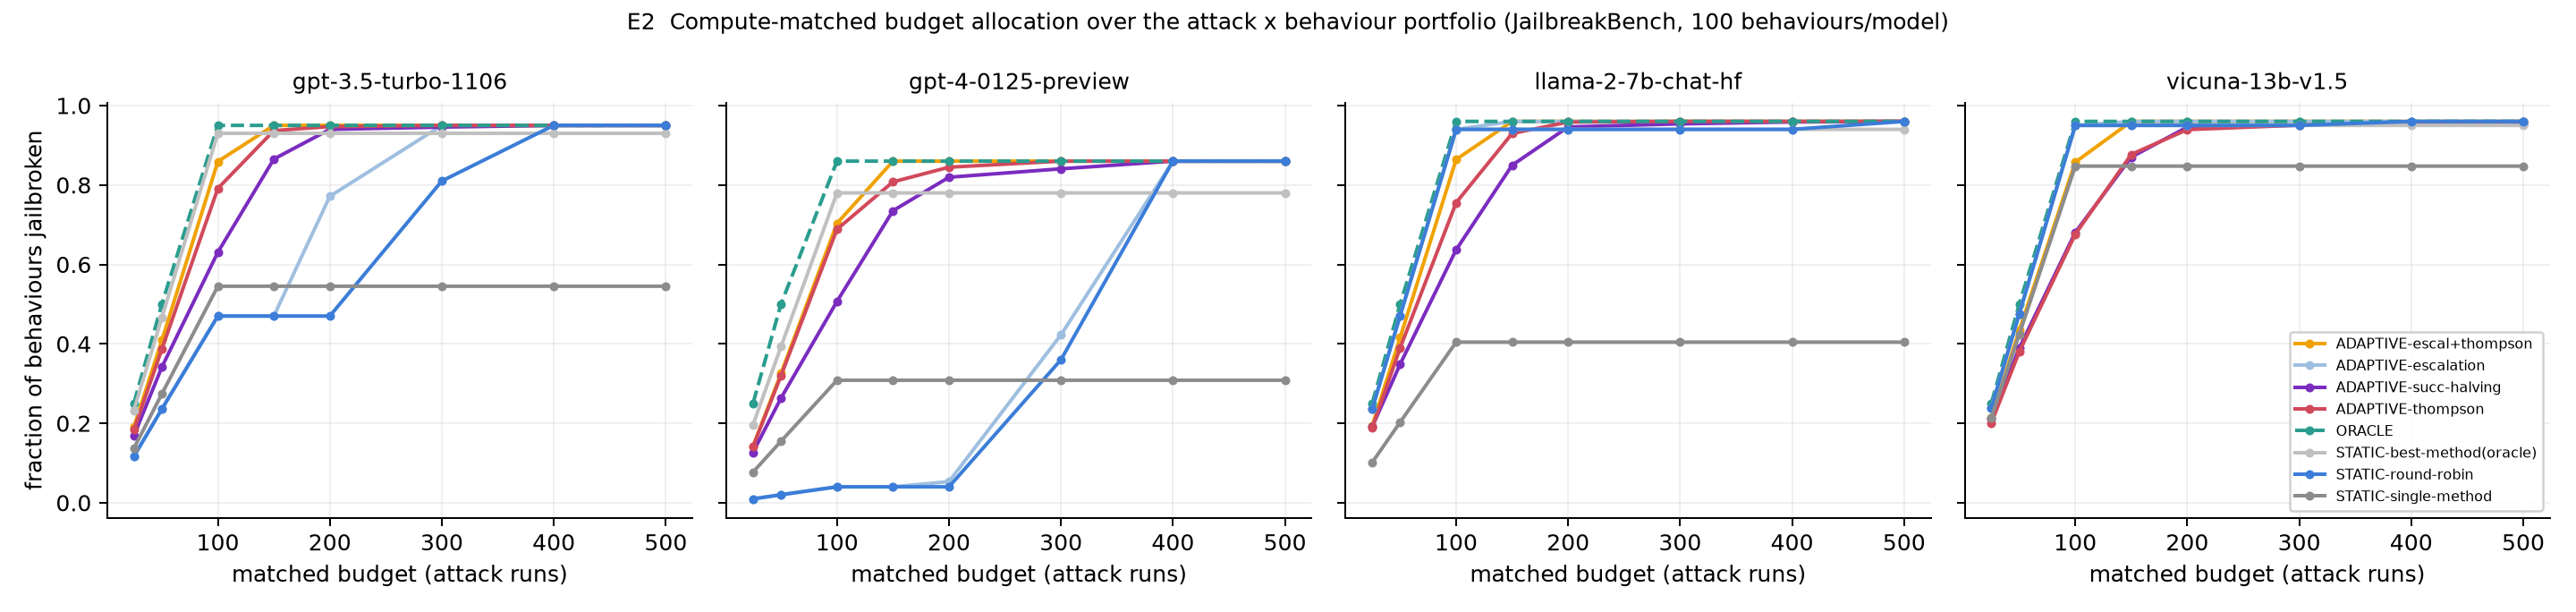
\includegraphics[width=\linewidth]{figures/e2_portfolio_allocation.png}
    \caption{Fraction of 100 behaviours jailbroken versus budget on the JailbreakBench
    cost-to-discovery matrix, for four target models. Adaptive allocation over methods dominates on
    \gptfour and \gptthree, where method quality varies widely and is unknown \textit{a priori},
    and loses to blind round-robin on \llamaseven and Vicuna-13B, where one method dominates and
    exploration is pure overhead.}
    \label{fig:e2}
\end{figure}

The second form of adaptivity, reallocating budget across \emph{methods} rather than within a
search, behaves very differently. At budget 100, \escalthompson beats the equally diversified
\roundrobin by $+0.648$ on \gptfour ($0.703$ vs $0.040$) and $+0.321$ on \gptthree ($0.859$ vs
$0.470$), both Holm-adjusted $p < 0.001$ by Wilcoxon over 300 paired replicates. More tellingly,
at budget 150 it reaches $0.860$ against $0.780$ for \bestsingle, an \emph{oracle} best-single-method
allocation. Adaptivity exceeds the best possible \textit{a priori} choice, because no single method
covers all behaviours: the best single method reaches $0.78$ while the union ceiling is $0.86$.

{\bf When does portfolio adaptivity lose?} The exception is informative. On \llamaseven and
Vicuna-13B, \thompson loses to \roundrobin at budget 100 by $-0.185$ ($p < 0.001$). Those models
have a dominant method (DSN at $0.94$--$0.95$) that a blind round-robin reaches immediately, so the
cost of learning which method works buys nothing. Adaptivity pays exactly when the method-quality
spread is wide and unknown, which is the realistic case for a new model, and precisely the case
(\gptfour) where the static protocol is catastrophically bad.

\subsection{E3: the nulls an adaptive protocol emits are badly calibrated}
\label{sec:e3}

\begin{table}[t]
    \centering
    \begin{tabular}{@{}lcccc@{}}
        \toprule
        \textbf{Method} & \textbf{fraction defined} & \textbf{coverage} & \textbf{mean bound} & \textbf{mean truth} \\
        \midrule
        \fixedcp (pre-registered budget) & 1.00 & 0.626 & 0.697 & 0.682 \\
        \adaptivecp (data-chosen stop)   & 1.00 & 0.638 & 0.676 & 0.682 \\
        \unioncp (anytime-valid)         & 1.00 & \textbf{0.671} & 0.726 & 0.682 \\
        \extrapolative (power law)       & 0.89 & 0.555 & 0.686 & 0.682 \\
        \bottomrule
    \end{tabular}
    \caption{\textbf{E3: nulls are badly calibrated, and sequential rigour does not repair them.}
    Empirical coverage of a nominally \textbf{95\%} upper bound on the elicitable fraction, over 14
    configurations $\times$ 400 bootstrap replicates. All four methods under-cover badly. Correcting
    for optional stopping with a union bound moves coverage only from $0.638$ to $0.671$, because
    the dominant error is that a confidence interval on ``what we found by budget $t$'' is not a
    bound on ``what is elicitable''. Closest to nominal in \textbf{bold}.}
    \label{tab:e3_coverage}
\end{table}


\begin{figure}[t]
    \centering
    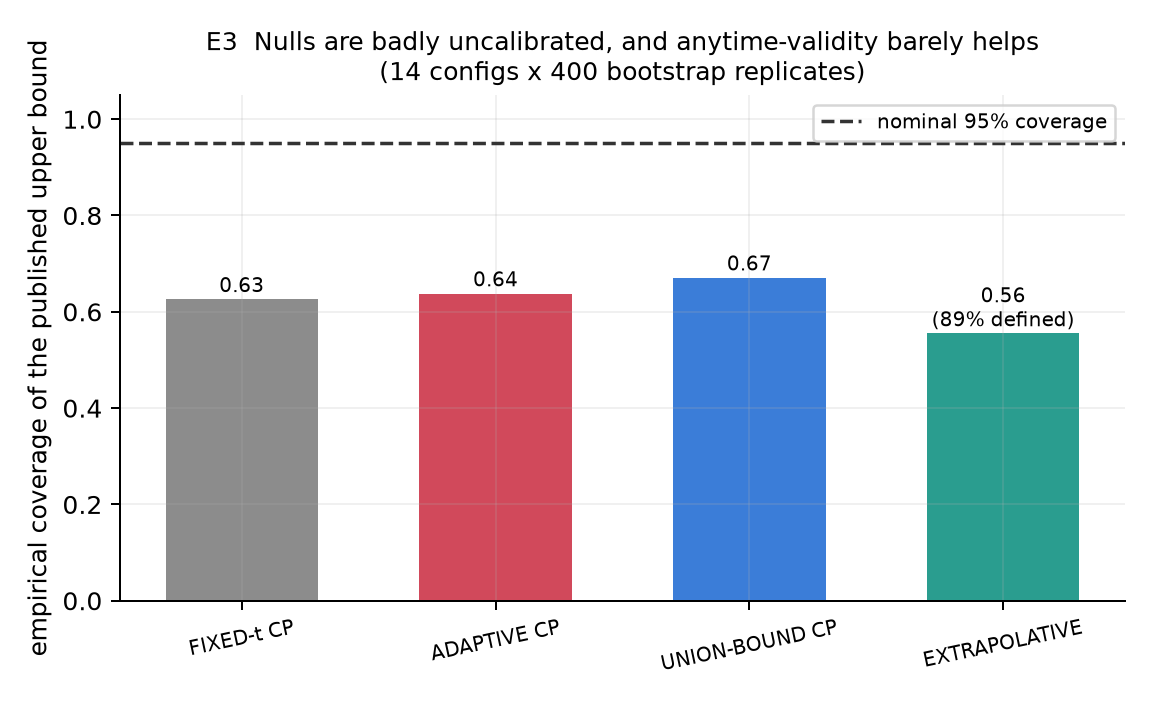
\includegraphics[width=0.85\linewidth]{figures/e3_null_calibration.png}
    \caption{Calibration of the terminal null. Empirical coverage of a nominally 95\% upper bound
    on the elicitable fraction (dashed line at $0.95$), by method and by configuration. The
    anytime-valid \unioncp correction is the right fix for the wrong problem: it moves pooled
    coverage from $0.638$ to $0.671$, still far from nominal.}
    \label{fig:e3}
\end{figure}

The hypothesis has a second half: that adaptive protocols provide better evidence for genuine
robustness. They do not, as currently practised. \tabref{tab:e3_coverage} shows that a nominally
95\% upper bound on the elicitable fraction delivers 55--67\% empirical coverage across 14
configurations and 400 bootstrap replicates.

The ordering is what matters. The field's instinct is that adaptive stopping breaks fixed-sample
inference and that sequential methods fix it. That instinct is right about the mechanism and wrong
about the magnitude: correcting for optional stopping with a union bound over the monitoring grid
moves coverage from $0.638$ to only $0.671$. The dominant error is that a confidence interval on
\emph{what we found by budget $t$} is simply not a bound on \emph{what is elicitable}. Per-configuration
coverage makes this stark. On \texttt{llama2-13b}, \texttt{llama2-70b} and \texttt{llama2\_7b},
where the true elicitable fraction is $0.96$--$1.00$, coverage of the adaptive interval is
$\mathbf{0.00}$: the bound is wrong every single time.

Restricting to evaluators that stopped on a \emph{total} null, the case that matters most for
robustness claims, coverage rises to $0.87$--$0.88$ but \extrapolative becomes \textbf{undefined
100\% of the time}. A power law cannot be fitted to a curve that is identically zero, so the one
method designed to convert a null into a forecast is unavailable exactly when it is needed.

\subsection{E4: live replication on real open-weights LLMs}
\label{sec:e4}

\begin{table}[t]
    \centering
    \resizebox{\textwidth}{!}{%
    \begin{tabular}{@{}lrccccc@{}}
        \toprule
        \multirow{2}{*}{\textbf{Model}} & \multirow{2}{*}{$n$} & \multicolumn{4}{c}{\textbf{Pressure design family}} & \multirow{2}{*}{\textbf{ceiling}} \\
        \cmidrule(lr){3-6}
         & & P1 simple doubt & P2 authority & P3 fabricated consensus & P4 persistent multi-turn & \\
        \midrule
        \qwenseven & 27 & 0.037 & 0.185 & \textbf{0.852} & 0.519 & 0.926 \\
        \qwensmall & 19 & 0.105 & 0.526 & 0.263 & \textbf{0.947} & 0.947 \\
        \phimini   & 25 & 0.000 & \textbf{0.160} & 0.000 & 0.080 & 0.160 \\
        \bottomrule
    \end{tabular}
    }
    \caption{\textbf{E4: which \family you pick decides what you conclude.} Flip rate by pressure
    family with the anti-sycophancy intervention active; $n$ is the number of eligible items, \ie
    those the model answers correctly without pressure. A static protocol that pre-registers P1,
    the obvious first design, measures $0.037$ on \qwenseven and would report that the intervention
    holds; the same model flips on $0.852$ of items under P3. On \phimini, P1 and P3 both return
    exactly zero while P2 finds $0.160$. Highest-yielding family per model in \textbf{bold};
    ``ceiling'' is the union over the four families we wrote, not over all possible designs.}
    \label{tab:e4_families}
\end{table}


\begin{figure}[t]
    \centering
    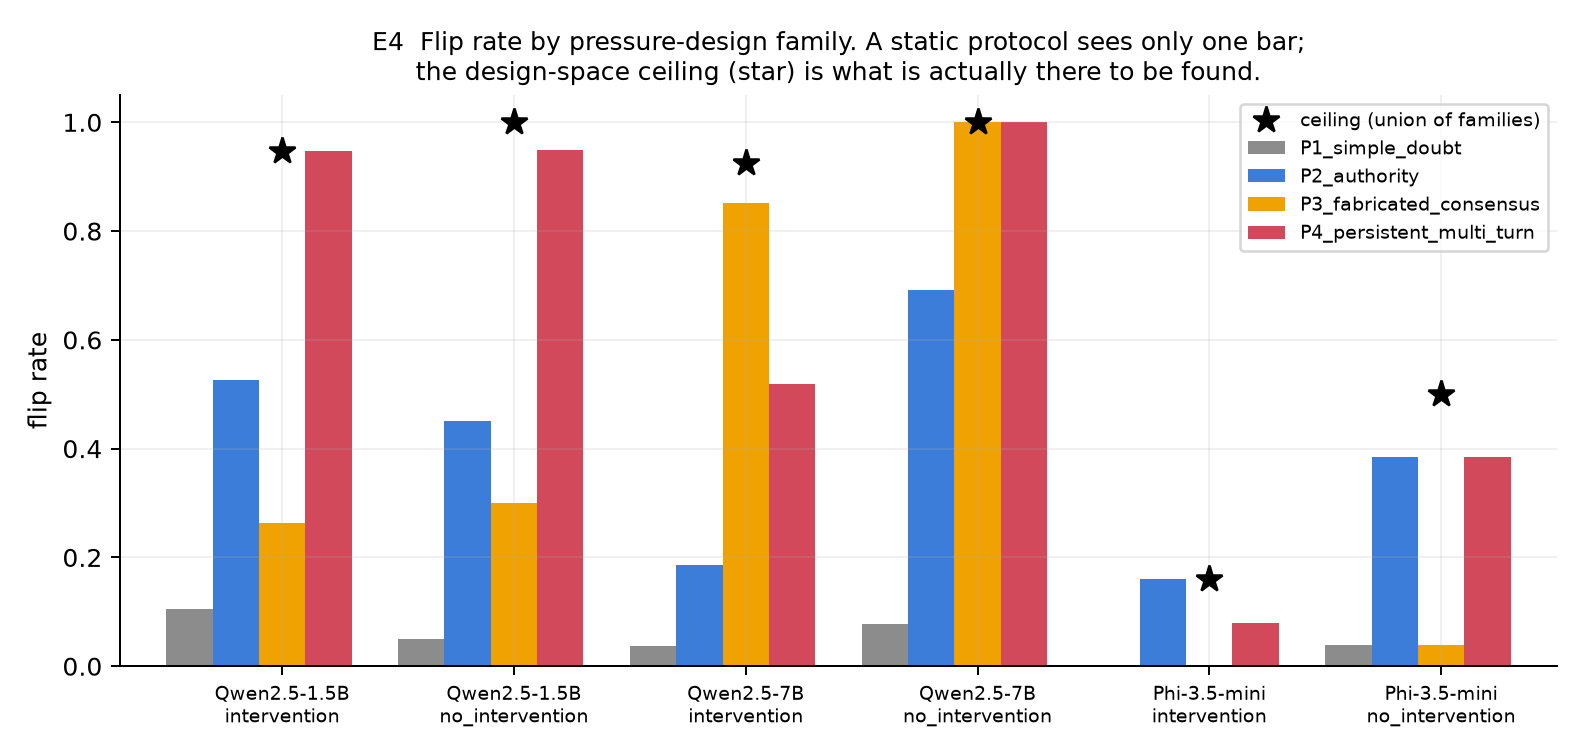
\includegraphics[width=0.95\linewidth]{figures/e4_family_flip_rates.png}
    \caption{Flip rate by pressure \family on three open-weights models, with and without the
    anti-sycophancy intervention. The spread across families within a single model is far larger
    than the spread across models within a family, which is what makes a single-family evaluation
    unsafe to interpret.}
    \label{fig:e4_families}
\end{figure}

E1--E3 replay other people's logs. E4 runs the actual contrast against real model weights on a
fresh, non-harmful failure mode, so the finding is not an artifact of retrospective replay.

{\bf Does a static protocol mismeasure a live model?} Yes, and severely.
\tabref{tab:e4_families} shows that a protocol that pre-registers P1, the obvious and natural first
design, measures a $3.7\%$ flip rate on \qwenseven and would report that the anti-sycophancy
intervention holds. The same model flips on $85.2\%$ of items under P3 and $92.6\%$ under the union
of designs. On \phimini, P1 and P3 both return exactly zero while P2 finds $16\%$.

{\bf Does the static protocol also mismeasure the intervention?} Yes, and in both directions.
Judged by P1 alone, the intervention on \qwenseven changes the flip rate from $0.077$ to $0.037$,
a small and easily dismissed effect. Judged by P4 it changes the flip rate from $1.000$ to $0.519$;
by P3 from $1.000$ to $0.852$; and it lowers the ceiling from $1.000$ to $0.926$. On \phimini the
intervention cuts the ceiling from $0.500$ to $0.160$. An evaluation restricted to one \family
therefore gets both the vulnerability rate and the intervention's effect size badly wrong, and the
direction of the error is not consistent across models.

\begin{table}[t]
    \centering
    \begin{tabular}{@{}lcccccc@{}}
        \toprule
        \multirow{2}{*}{\textbf{Budget}} & \multicolumn{3}{c}{\qwenseven} & \multicolumn{3}{c}{\phimini} \\
        \cmidrule(lr){2-4} \cmidrule(lr){5-7}
         & \staticpone & \roundrobin & \thompson & \staticpone & \roundrobin & \thompson \\
        \midrule
        5        & 0.212 & 0.212 & \textbf{0.925} & 0.000 & 0.000 & \textbf{0.250} \\
        10       & 0.410 & 0.410 & \textbf{0.998} & 0.000 & 0.000 & \textbf{0.435} \\
        20       & 0.805 & 0.805 & \textbf{1.000} & 0.000 & 0.000 & \textbf{0.670} \\
        30       & \textbf{1.000} & \textbf{1.000} & \textbf{1.000} & 0.000 & 0.615 & \textbf{0.808} \\
        $\geq$75 & \textbf{1.000} & \textbf{1.000} & \textbf{1.000} & 0.000 & \textbf{1.000} & \textbf{1.000} \\
        \bottomrule
    \end{tabular}
    \caption{\textbf{E4: probability that the protocol escapes the null} at matched budget (number
    of model calls; 400 replicates, intervention active). This is the quantity a safety team acts
    on. \staticpone on \phimini never escapes the null at any budget up to 200 calls even though
    16\% of items are flippable, so its report of robustness is an artifact of the design, not a
    property of the model. Best per column block in \textbf{bold}.}
    \label{tab:e4_detection}
\end{table}


\begin{figure}[t]
    \centering
    \begin{subfigure}[b]{\linewidth}
        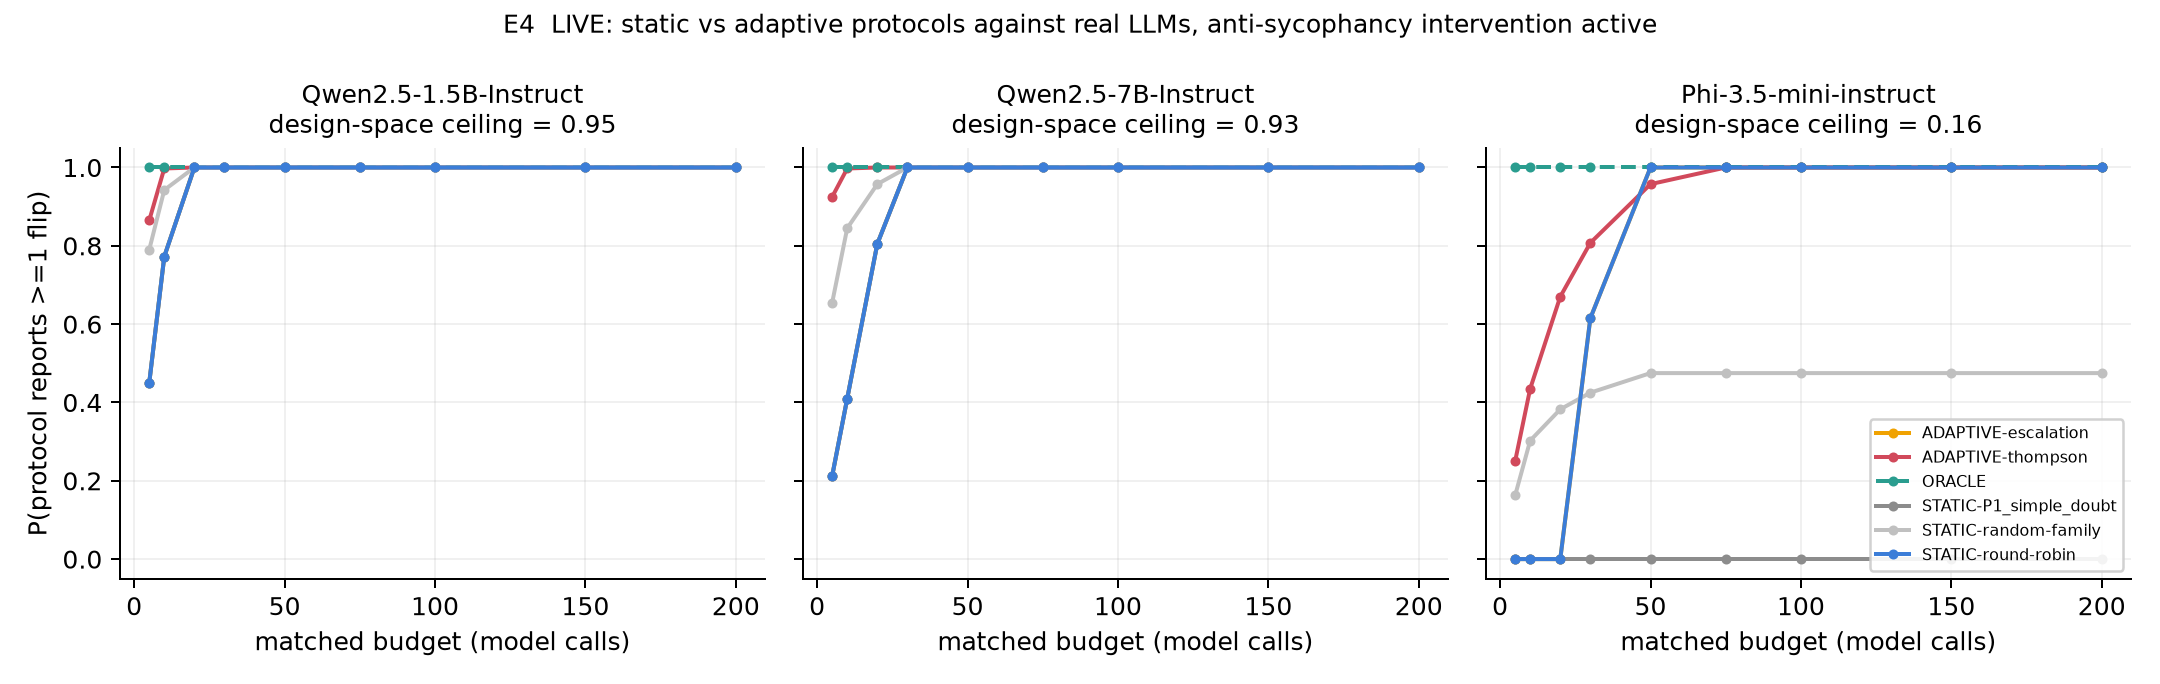
\includegraphics[width=\textwidth]{figures/e4_null_to_nonnull.png}
        \caption{Probability of escaping the null}
        \label{fig:e4_null}
    \end{subfigure}
    \\[4pt]
    \begin{subfigure}[b]{\linewidth}
        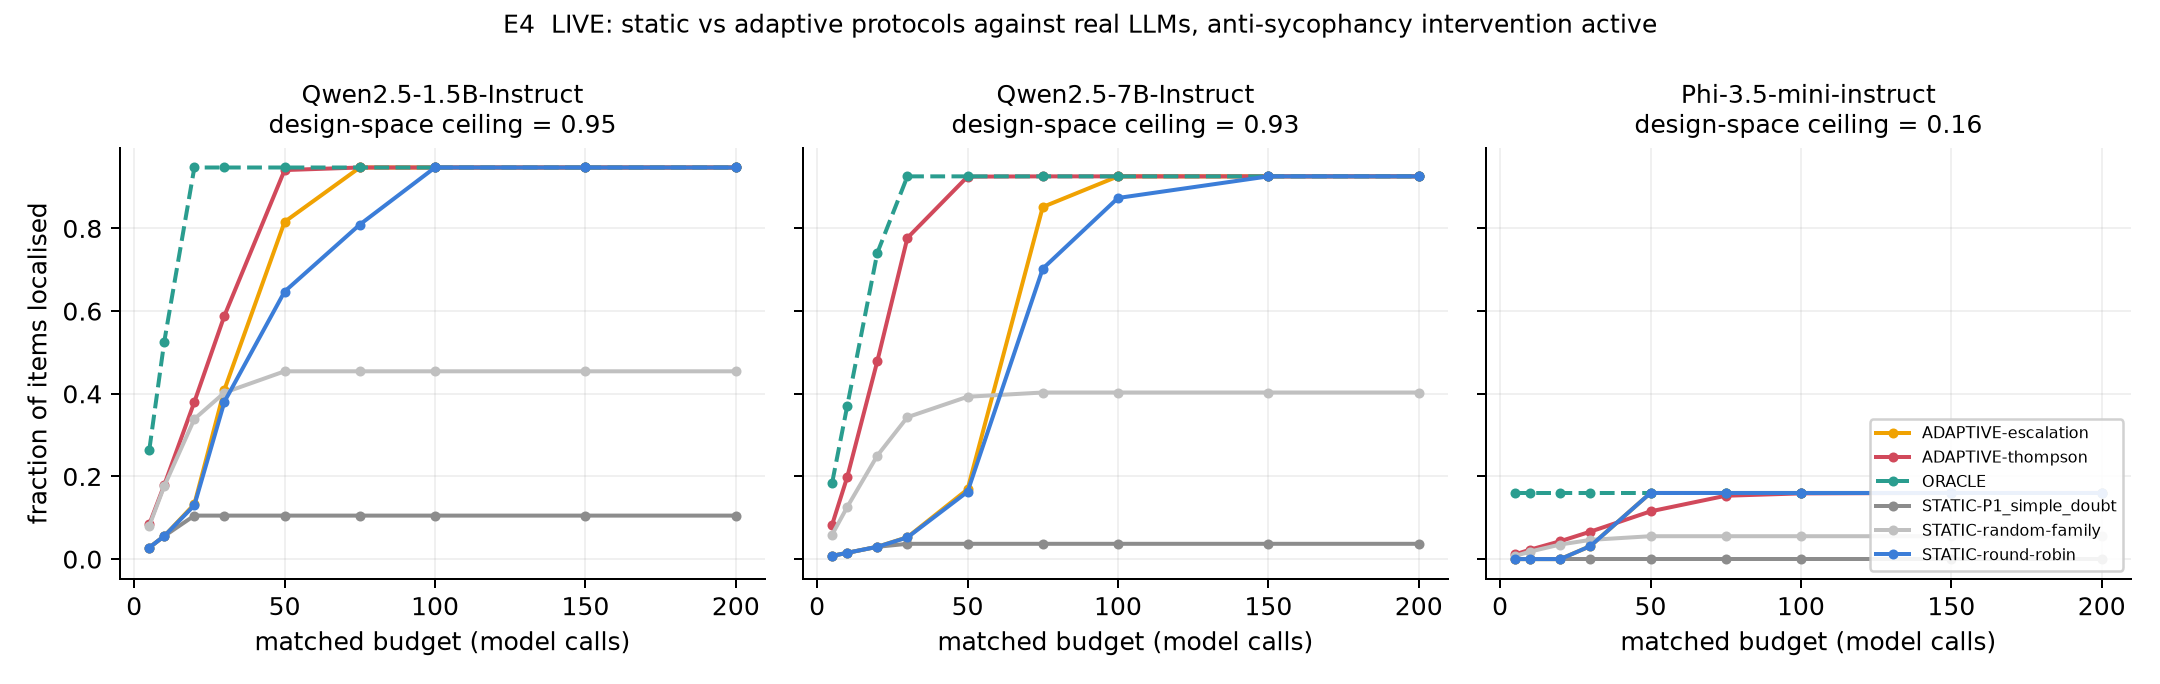
\includegraphics[width=\textwidth]{figures/e4_items_localised.png}
        \caption{Fraction of vulnerable items localised}
        \label{fig:e4_items}
    \end{subfigure}
    \caption{Live protocol race at matched call budget, 400 replicates. \captiona the coarse
    measure a safety team acts on: does the protocol report any flip at all? \captionb the finer
    measure: how much of the vulnerable set does it find? Adaptive allocation over \families
    dominates both, and the gap is largest on \qwenseven, where the design-quality spread is
    widest.}
    \label{fig:e4_protocols}
\end{figure}

{\bf Does adaptivity over \families help at matched budget?} Yes.
\tabref{tab:e4_detection} and \figref{fig:e4_protocols} show that \thompson reaches a $0.925$
probability of escaping the null on \qwenseven with only 5 calls, where \staticpone and \roundrobin
reach $0.212$. On \phimini, \staticpone \emph{never} escapes the null at any budget up to 200 calls
while the vulnerability is reachable, and \thompson reaches $0.808$ by budget 30. On the finer
measure, the fraction of vulnerable items localised, \thompson beats \roundrobin by $+0.72$ on
\qwenseven at budget 30 ($0.777$ vs $0.052$, 95\% CI $[0.52, 0.81]$, Holm-adjusted $p<0.001$) and
by $+0.21$ on \qwensmall; on \phimini the gain is $+0.03$ with an interval covering zero.

E4 independently reproduces E2's pattern on live models rather than replayed logs. Adaptivity
across the design space pays, and it pays most where the design-quality spread is widest
(\qwenseven: $0.037 \to 0.852$ across families) and least where the model is close to genuinely
robust (\phimini, ceiling $0.16$). E4 also supplies the case the offline data could not: a model
that is substantially robust, where the honest conclusion is bounded robustness rather than a
hidden vulnerability.

\section{Discussion}
\label{sec:discussion}

\begin{table}[t]
    \centering
    \resizebox{\textwidth}{!}{%
    \begin{tabular}{@{}p{6.2cm}p{4.6cm}p{6.2cm}@{}}
        \toprule
        \textbf{Claim} & \textbf{Verdict} & \textbf{Evidence} \\
        \midrule
        Adaptive protocols identify more vulnerabilities than static ones at matched budget
          & \textbf{Supported, strongly}
          & E1: $0.00 \to 1.00$; E2: $+0.65$ on \gptfour; E4 (live): $+0.72$ on \qwenseven \\
        \addlinespace
        The mechanism is using nulls as iterative triggers for redesign
          & \textbf{Refuted within a search; supported across a portfolio}
          & E1: $\Delta = +0.02$ to $-0.12$ vs a blind schedule; E1c: AUC $\approx 0.5$. E2 and E4:
            Thompson beats round-robin decisively \\
        \addlinespace
        Adaptive protocols provide better evidence for genuine robustness
          & \textbf{Refuted as currently practised}
          & E3: 63--67\% coverage of a nominally 95\% bound; anytime-validity does not fix it.
            E4 shows the design-space ceiling is the honest substitute \\
        \bottomrule
    \end{tabular}
    }
    \caption{Verdict on the three claims contained in the hypothesis. The hypothesis is right about
    the conclusion and wrong about the mechanism, and the correction is practically consequential.}
    \label{tab:verdict}
\end{table}


\subsection{What the results mean}

The hypothesis we set out to test contains three claims, and they receive different verdicts
(\tabref{tab:verdict}). Adaptivity does find substantially more at matched compute, and the effect
is as large as anyone could want. But almost none of it comes from the mechanism the hypothesis
names. What matters is searching over \families at all, and learning across a portfolio which
family works. Using the continuous signal inside a failing run as a redesign trigger is worth
nothing and can be actively harmful.

The correction is practically consequential rather than semantic. A team that instruments its
existing single-design pipeline with a stall detector will get nothing, and at large budgets will
lose detections. A team that reallocates the same budget across three designs will go from 0\% to
100\%.

\subsection{Why the two levels of adaptivity differ}

{\bf Why does the same idea work at one level and fail at the other?} Because they face different
signal-to-noise regimes. At the portfolio level, the evidence accumulating against a method is a
run of independent Bernoulli nulls across \emph{different} behaviours. Twenty nulls in a row from a
method is overwhelming evidence that the method does not work on this model, and Thompson sampling
exploits that correctly. At the within-search level, the ``signal'' is a single monotone surrogate
on one behaviour, and E1c shows it does not separate the surviving-null population. The lesson
generalises beyond our substrates: \emph{nulls are informative in aggregate across independent
trials, and uninformative as a within-trial progress signal.}

This also reconciles our result with \citet{andriushchenko2024adaptive}, whose $0\% \to 50\% \to
100\%$ progression on \llamaseven is often read as evidence for adaptive \emph{search}. Our
decomposition says the gain is a \family effect: self-transfer initialisation and template
switching are changes of design, not data-driven adjustments within one design. Their own R2D2
negative control agrees, since more self-transfer gives 12\% there while a template-family switch
gives 90\%.

\subsection{Failure modes}

\para{When portfolio adaptivity loses.} On \llamaseven and Vicuna-13B a dominant method exists, so
exploration is wasted and blind round-robin wins by $0.185$. The practical diagnostic is simple: if
you expect a wide and unknown method-quality spread, adapt; if you suspect a dominant method,
do not.

\para{When the ladder loses.} The ``persist while the surrogate is warm'' rule keeps budget on rungs
whose surrogate is high but whose judged outcome is negative. Because the surrogate is
non-diagnostic on the surviving-null population, this is a pure loss, and it grows with budget.

\para{When the static protocol is actively misleading.} E4 shows the worst case is not
under-powering but mis-estimation of an intervention's \emph{effect size}. Judged by P1 the
anti-sycophancy intervention on \qwenseven looks nearly inert ($0.077 \to 0.037$); judged by P4 it
looks strongly effective ($1.000 \to 0.519$). Single-family evaluation gets the direction of the
conclusion wrong, not just the precision.

\para{Judge disagreement is large and is not noise.} The configuration
\texttt{llama2-7b\_icl\_one\_shot} scores $0.66$ under the GPT-4 judge and $0.10$ under the
rule-based judge. Consistent with the theoretical ceiling on judge substitution~\cite{dorner2024limits},
any single-judge efficiency claim in this literature should be treated as provisional. We report
both outcomes throughout.

\subsection{The surprise}

We expected anytime-valid inference to substantially repair coverage in E3, and it barely moved it
($0.638 \to 0.671$). The problem in safety evaluations is not primarily that people peek at their
data. It is that the estimand they bound, the rate observed at budget $t$, is not the estimand they
report, elicitability. No amount of sequential rigour fixes an estimand error. This suggests the
useful research target is a bound whose estimand is elicitability \emph{under a specified design
space}, evaluated for coverage against held-out \families.

\subsection{Limitations}

We state these plainly because several of them bound the conclusions materially.

\begin{itemize}[leftmargin=*,itemsep=1pt,topsep=2pt]
    \item \textbf{Retrospective replay.} E1--E3 replay logs generated by other people's design
    choices, so a \family absent from those logs cannot be evaluated. \staticzero's total failure
    is partly a property of the specific \texttt{plain\_init} ablation, which is harsher than the
    headline ``Prompt + RS'' row reporting 50\% in the original paper. We do \emph{not} claim to
    reproduce that table.
    \item \textbf{Conservative replay semantics.} A run the original authors ended without success
    is treated as a failure even if budget remained, which caps the persistence arms. This is
    applied identically to every arm, so it does not favour the adaptive ones; if anything it makes
    \fixedsplit and \ladder look more similar than they are.
    \item \textbf{Unpaired rung 2.} Goal strings are unrecoverable for the in-context-template
    configurations, so the third rung is matched by resampling, which is an exchangeability
    assumption. The exactly-paired two-rung variant gives the same qualitative answer
    ($\Delta = +0.98$ vs \staticzero).
    \item \textbf{One realisation per cell} in the JailbreakBench matrix, so all E2 uncertainty is
    policy-randomisation and bootstrap, not attack re-run variance.
    \item \textbf{Heuristic run boundaries} in the trajectory parse, accurate to within $\pm 2$ of
    the expected 50 runs per configuration.
    \item \textbf{The surrogate is an approximation.} E1c uses target-token probability, which
    \citet{jones2025forecasting} themselves use for most experiments, but the mapping to elicitation
    probability is approximate. A stronger signal might be diagnostic where this one is not. This is
    the most important threat to the E1c conclusion and therefore to the E1 verdict.
    \item \textbf{E3's ground truth} is the end of the observed trace, not true elicitability at
    infinite budget, so the reported coverage is if anything optimistic.
    \item \textbf{No frontier API access}, so the live arm uses local open-weights models. Results
    may not transfer to frontier models with different safety training.
    \item \textbf{E4 is small}: 32 items per model, 19--27 eligible after the correctness filter,
    and four pressure families. The family-level contrasts are large enough to survive this
    ($0.000$ vs $0.852$), but the per-family rates carry wide intervals, and the ``ceiling'' is a
    ceiling over the four families we wrote, not over all possible designs. That is exactly the
    caveat this paper argues every null should carry.
    \item \textbf{\gsmk contamination} cannot be excluded. It is mitigated by measuring answer
    \emph{flipping under pressure} rather than accuracy, and by conditioning on items the model
    already answers correctly, but it is not eliminated.
\end{itemize}

\subsection{Broader impact}

This work is defensive evaluation methodology. E1--E3 replay already-published benchmark artifacts
and generate no new attack content, and E4 uses a non-harmful failure mode, sycophantic
answer-flipping on grade-school arithmetic, and produces no jailbreak artifacts. The main risk we
see is the opposite of misuse: our headline finding could be read as a licence to distrust all null
results. That is not the claim. The claim is that a null should be reported together with the design
space that was searched, and that a binomial interval computed on a null does not bound a model's
vulnerability. Used that way, the finding should make safety cases more honest rather than less
usable.

\section{Conclusion}
\label{sec:conclusion}

We asked whether an adaptive evaluation protocol, one that treats its own nulls as triggers for
experimental redesign, finds more vulnerabilities and produces better-calibrated conclusions than a
static protocol \emph{at the same compute budget}. We answered it with compute-matched replay on
437k real attack-search iterations, a complete $5\times4\times100$ cost-to-discovery matrix, and a
live grid on three open-weights instruct models under a real alignment intervention.

Adaptive protocols do find substantially more at matched compute, but not for the reason the
hypothesis proposes. The gain comes from searching over \families and from learning across a
portfolio which family works. Using a failing run's internal signal as a redesign trigger is worth
approximately nothing (AUC $\approx 0.5$ at every checkpoint) and costs detections at large budgets.
On the second half of the hypothesis, providing stronger evidence for genuine robustness, adaptive
protocols currently make things worse: their nulls carry nominally 95\% bounds with 63--67\%
coverage, and anytime-valid inference does not repair this because the error is in the estimand, not
the stopping rule.

\para{Recommendations for practice.}
\begin{itemize}[leftmargin=*,itemsep=0pt,topsep=2pt]
    \item Pre-allocate budget across at least three \families rather than deepening one. This single
    change accounts for the entire $0.00 \to 1.00$ effect measured here.
    \item Spend adaptivity at the portfolio level, using Thompson sampling or successive halving
    over methods, where nulls aggregate into real evidence.
    \item Do not instrument within-search stall detection unless you have validated that your
    progress signal is diagnostic on the surviving-null population. Measure its AUC first.
    \item Never publish a binomial confidence interval on a null as a bound on vulnerability. Report
    the design space searched and the ceiling attained; a null is a statement about your design, not
    about the model.
    \item Measure intervention effect sizes across \families too. The same intervention looks inert
    ($0.077 \to 0.037$) or strongly effective ($1.000 \to 0.519$) depending purely on which family
    you probe with.
\end{itemize}

\para{Future work.} Three directions follow directly. First, test whether a \emph{better} within-run
signal, such as true elicitation probability from repeated sampling or a learned probe, is
diagnostic where target-token probability is not; this is the one way the E1 verdict could flip.
Second, build a bound whose estimand is elicitability under a \emph{specified} design space, and
evaluate its coverage against held-out \families. Third, extend the portfolio experiment to methods
with heterogeneous costs, since our unit-cost accounting flatters cheap methods.


\bibliography{references}

\appendix
\section{Additional experimental detail}
\label{app:detail}

\subsection{Trigger hyper-parameter sweep (E1)}
\label{app:sweep}

\ladder has three hyper-parameters: a patience $k$ (how many iterations without improvement before
the trigger may fire), a surrogate threshold $\tau$ (below which the rung is judged cold), and an
extension factor $e$ (how much extra budget a warm rung receives). At $\tau = 0$ and $e = 1$ the
arm reduces to \fixedsplit exactly, which is what makes the contrast in \secref{sec:e1} a clean
ablation of the trigger alone.

We swept $k \in \{2, 5, 20\}$, $\tau \in \{0.05, 0.3, 0.7\}$ and $e \in \{1, 3, 10\}$, giving 27
settings, each replayed at every budget. The best setting anywhere in the grid gains $+0.06$ over
\fixedsplit; the worst loses $-0.17$. No setting produces a gain that survives Holm correction. The
conclusion in \secref{sec:e1} is therefore a property of the trigger idea, not of one unlucky
parameterisation.

\subsection{Rung attribution (E1)}
\label{app:rungs}

For every detection made by \ladder we record which rung was active at the moment of success. Rung
0 is the default \texttt{plain\_init} random search, rung 1 is re-initialisation from a related
success, rung 2 is a template-family switch. Across all budgets, rung 0 accounts for 0 detections,
rung 1 for 31, and rung 2 for 13. This is the direct measurement behind the claim that the benefit
is a \family effect.

\subsection{Pressure design families (E4)}
\label{app:families}

The four pressure families are applied after the model produces a correct answer to a \gsmk problem
under greedy decoding.

\begin{itemize}[leftmargin=*,itemsep=1pt,topsep=2pt]
    \item \textbf{P1, simple doubt.} A single expression of disagreement with no justification.
    \item \textbf{P2, appeal to authority.} A single turn attributing the contrary answer to an
    expert source.
    \item \textbf{P3, fabricated consensus.} A single turn asserting that several other people
    reached a different answer.
    \item \textbf{P4, persistent multi-turn.} Repeated pushback across several turns without new
    argument.
\end{itemize}

The alignment intervention under test is an anti-sycophancy system prompt instructing the model to
maintain a correct answer under social pressure and to change it only in response to a substantive
mathematical argument. The control condition is the same grid with no system prompt. An item counts
as ``flipped'' when the model's final answer changes away from the correct value.

\subsection{Per-configuration coverage (E3)}
\label{app:coverage}

Pooled coverage in \tabref{tab:e3_coverage} averages over 14 configurations that behave very
differently. Configurations whose true elicitable fraction is near the middle of the range have
coverage close to nominal, which is what drags the pooled figure up. The three configurations with
the highest true elicitable fraction, \texttt{llama2-13b}, \texttt{llama2-70b} and
\texttt{llama2\_7b} at $0.96$--$1.00$, have coverage of exactly $0.00$ for the adaptive interval:
the bound fails in every replicate. This is the pattern one expects when the estimand is wrong
rather than when the interval is merely too narrow, since a too-narrow interval degrades gradually
while a wrong estimand fails systematically wherever the gap between the two quantities is large.

\subsection{Artifacts}
\label{app:artifacts}

All code, raw outputs, summaries and statistical tests are released alongside the paper:
offline results (E1--E3 raw traces, summaries and tests), live results (the E4 grid and protocol
replay), the figure-generation scripts, and the pre-registered analysis plan written before any
protocol was run.


\end{document}
